%%%%%%%%%%%%%%%%%%%%%%%%%%%%%%%%%%%%%%%%%%%%%%%%%%%%%%%%%%%%%%%%%%%%%%%%%%%%%%%%
%neutrino_physics.tex: Chapter on neutrino physics:
%%%%%%%%%%%%%%%%%%%%%%%%%%%%%%%%%%%%%%%%%%%%%%%%%%%%%%%%%%%%%%%%%%%%%%%%%%%%%%%%
\chapter{Theoretical Motivations}
\label{wrBosonAndHeavyNu}
%%%%%%%%%%%%%%%%%%%%%%%%%%%%%%%%%%%%%%%%%%%%%%%%%%%%%%%%%%%%%%%%%%%%%%%%%%%%%%%%
Experimental evidence of massive neutrinos and the baryon-antibaryon asymmetry motivates extensions to the ST.  
In this chapter, the ST description of particle mass generation is discussed as a precursor to ST extensions.  
Then, the Majorana neutrino model and generic LRS models are explained, and highlighting how these extensions 
show better agreement with experimental observations than the ST.  Finally, this chapter concludes with 
important characteristics of LRS models that can be studied at the LHC, and a predicted experimental signature 
shown in Figure \ref{fig:wrFeynmanDiagram}.

\begin{figure}[h]
	\centering
	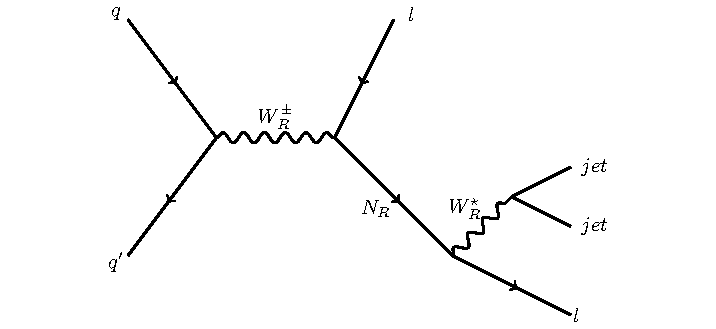
\includegraphics[width=1.0\textwidth]{figures/feynman.pdf}
	\caption{Production of a \WR boson and its decay to two charged leptons and two quarks through 
	a heavy neutrino \nul.}
	\label{fig:wrFeynmanDiagram}
\end{figure}


\section{Particle Masses in the Standard Theory}
\label{sec:massInSM}
The ST postulates that the four generators of the $SU(2)_{L} \times U(1)$ groups transform into the massless 
photon and massive $W^{\pm}$ and $Z$ bosons through the Brout-Englert-Higgs (BEH) mechanism.  This mechanism 
introduces a complex doublet $\Phi$, representing four scalar bosons, that obey the Lagrangian $\Ell_{H}$:

\begin{align}
	\Phi &= \begin{bmatrix}
	\phi^{+} \\
	\phi^{0}
	\end{bmatrix}
\end{align}

\begin{equation}
	\Ell_{H} = (D_{\mu}\Phi)^{\dagger}D^{\mu}\Phi - V(\Phi)
\end{equation}

where $V(\Phi) = \frac{1}{2}(|\Phi|^{2} - \frac{\nu^{2}}{2})$ is the Higgs potential (see Figure \ref{fig:smHiggsPotential}), and 
$D_{\mu} = \partial_{\mu} + ig_{L}\tau^{j}A^{j}_{\mu} + i\frac{g'}{2}YB_{\mu}$ describes the propagation 
of the Higgs doublet $\Phi$ and its couplings to the $SU(2)_{L}$ and $U(1)$ generators $\tau^{j}$ and $Y$, 
and to the massless vector fields $A^{j}_{\mu}$ and $B_{\mu}$.  $g_{L}$ and 
$g'$ set the weak and electromagnetic interaction coupling strengths.  The Higgs doublet $\Phi$ naturally 
moves to a value $<\Phi> =$ (0  $\nu/\sqrt{2}$) to minimize the Higgs potential, after which $\Ell_{H}$ reduces 
to:

\begin{figure}[h]
	\centering
	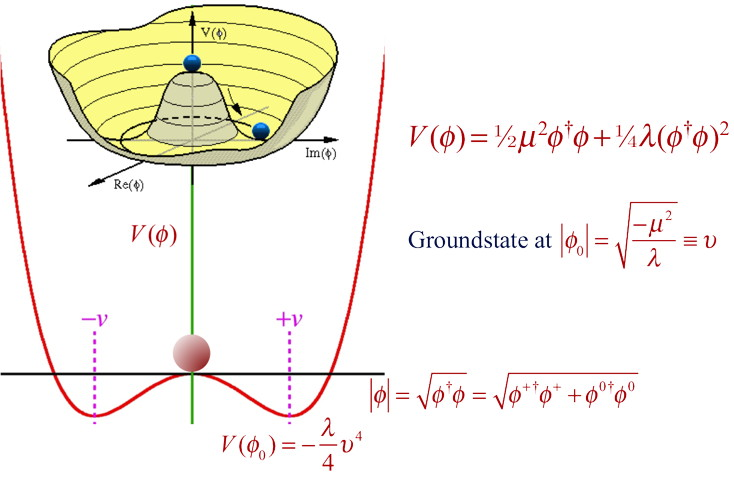
\includegraphics[width=1.0\textwidth]{figures/mexicanHatPotential.jpg}
	\caption{The Higgs potential drives the ST Higgs field to a stable state with non-zero vacuum expectation value, from $Swiss Physical Society$ \cite{higgsPotential}.}
	\label{fig:smHiggsPotential}
\end{figure}

\begin{equation}
	\Ell_{HK} = \frac{\nu^{2}}{8}[g^{2}_{L}(A^{1}_{\mu} + iA^{2}_{\mu})(A^{1\mu} - iA^{2\mu}) + (g'B_{\mu} - g_{L}A^{3}_{\mu})^{2}]
\end{equation}

Defining the photon vector field $A_{\mu}$, and the weak boson vector fields $W^{\pm}_{\mu}$ and $Z_{\mu}$ as:

\begin{equation}
	W^{\pm}_{\mu} \equiv \frac{1}{\sqrt{2}}(A^{1}_{\mu} \pm iA^{2}_{\mu}), 
	Z_{\mu} \equiv \frac{1}{\sqrt{g'^{2} + g^{2}_{L}}}(g'B_{\mu} - g_{L}A^{3}_{\mu}), 
	A_{\mu} \equiv \frac{1}{\sqrt{g'^{2} + g^{2}_{L}}}(g_{L}B_{\mu} + g'A^{3}_{\mu})
\end{equation}

transforms $\Ell_{H}$ into:

\begin{equation}
	\Ell_{HK} = (\frac{\nu g_{L}}{2})^{2}W^{+}_{\mu}W^{-\mu} + \frac{1}{2}(\frac{\nu \bar{g}}{2})^{2}Z_{\mu}Z^{\mu} + 0A_{\mu}A^{\mu}
\end{equation}

where $\bar{g} \equiv \sqrt{g'^{2} + g^{2}_{L}}$.  Following from this Lagrangian, the photon $A_{\mu}$ is massless, 
the $Z$ boson has mass $m_{Z} = \nu\bar{g}/2$, and the $W^{\pm}$ bosons have mass $m_{W} = \nu g_{L}/2$.  
Three of the four scalar fields introduced by the BEH mechanism are consumed to give mass to the $Z$ 
and $W^{\pm}$ bosons.  Recent experimental evidence of the fourth scalar field \cite{combinedHiggsResult}, the Higgs boson, 
supports the ST prediction that the $Z$ and $W^{\pm}$ bosons acquire mass through the BEH mechanism.

Experimental evidence indicates that quarks and charged leptons are massive fermions.  In the ST, fermions 
can acquire mass by adding mass terms directly to the ST Lagrangian, or by adding more Higgs fields to the 
BEH mechanism.  In either case, mass terms of the form $-mf\bar{f}$, where $f$ is a fermion, are added to 
the ST Lagrangian.  In the basis where a fermion field $f$ consists of right and left-handed components $\chi_{R}$ 
and $\chi_{L}$, $f = (\chi_{L},\chi_{R})$, a fermion mass term in the ST Lagrangian is expressed as:

\begin{equation}
	\Ell_{D} = -m\bar{f}f = -m\chi^{\dagger}_{L}\chi_{R} - m\chi^{\dagger}_{R}\chi_{L}
\end{equation}

This type of mass term, called a Dirac mass, contains the product of left and right-handed fields.  Experimental 
evidence substantiates that quarks and charged leptons exist in left and right-handed states that are degenerate 
in mass, so Dirac mass terms are used to assign masses to fermions in the ST.

Neutrinos play a special role in the ST.  The ST predicts that they are neutral, massless fermions, and only interact 
through the weak interaction.  In addition, due to parity violation of the weak interaction, 
anti-neutrinos $\bar{\nu_{\ell}}$ are always right-handed, and neutrinos $\nu_{\ell}$ are always left-handed.  
The ST can only assign masses to fermions using Dirac mass terms, which depend on the product of left and 
right-handed fields.  A Dirac mass term for neutrinos yields a mass of zero, so a ST extension is needed 
to model the experimental observation of massive neutrinos.


\section{Standard Theory Extensions}
\label{sec:lrsExtensions}
The ST can be extended in several ways to accommodate massive, fermionic neutrinos.  One of the simplest 
extensions predicts that neutrinos are not Dirac fermions, but Majorana fermions.  First proposed\cite{majoranaTheory} 
in 1937, Majorana fermions are their own anti-particles, and have masses $m_{L},m_{R}$ defined by the 
Lagrangian $\Ell_{M}$:

\begin{equation}
	\Ell_{M} = -m_{L}\chi^{\dagger}_{L}\chi_{L} - m_{R}\chi^{\dagger}_{R}\chi_{R}
\end{equation}

The individual Majorana masses can be generated through an extended Higgs model, or adding terms of the 
form $\Ell_{M}$ directly to the ST Lagrangian.  However, if Majorana neutrinos existed in nature, then 
the double beta decay process could occur with no neutrinos.  Experimental evidence of neutrinoless double 
beta decay has not been found \cite{igexDblBetaDecay,gerdaDblBetaDecay}, so a different ST extension is 
needed to predict massive neutrinos.

LRS models also predict massive fermionic neutrinos, but are not as tightly constrained by experimental 
evidence as the Majorana neutrino model.
First proposed in 1974 \cite{earlyLRSModel}, LRS models predict that a precursor to the ST electroweak 
interaction existed in the very early universe, and it conserved parity and was mediated by seven massless 
gauge bosons.  An extension of the ST BEH mechanism transformed the seven massless gauge bosons 
into the massless photon, the ST weak bosons, and the heavier $W^{\pm}_{R}$ (\WR) and $Z'$ bosons.  
Discussed next is the mechanism through which the ST weak bosons, \WR and $Z'$ bosons acquired mass, 
and is followed by a discussion of neutrino masses in LRS models.

The LRS models considered here add a $SU(2)_{R}$ group to the ST electroweak $SU(2)_{L} \times U(1)$ groups.
Adding the $SU(2)_{R}$ group introduces three massless vector fields $\xi^{j}_{\mu}$, which become massive 
bosons through an extended version of the ST BEH mechanism.  The ST BEH mechanism is extended in two stages, 
and ultimately yields one massless and six massive gauge bosons that mediate electroweak interactions.  In 
the first stage \cite{lrsHiggsStageOne}, a chiral, complex Higgs doublet $\chi_{L,R}$ is introduced: 

\begin{align}
	\chi_{L,R} &= \begin{bmatrix}
	\chi^{+}_{L,R} \\
	\chi^{0}_{L,R}
	\end{bmatrix}
	\label{eq:stageOneVEV}
\end{align}

with bosonic fields that couple independently to left and right-handed gauge bosons.  The propagation and 
interaction of these fields with other massless bosons is described by the Lagrangian:

\begin{equation}
	\Ell_{H,LRS} = \frac{1}{2}(D_{\mu}\chi_{L})^{\dagger}D^{\mu}\chi_{L} + \frac{1}{2}(D_{\mu}\chi_{R})^{\dagger}D^{\mu}\chi_{R} - V(\chi_{L,R})
\end{equation}

where $D_{\mu} = \partial_{\mu} + ig_{L}\tau^{j}A^{j}_{L\mu} + ig_{R}\tau^{j}\xi^{j}_{R\mu} + i\frac{g'}{2}YB_{\mu}$ contains 
the massless boson fields $A^{j}_{L\mu}, \xi^{j}_{R\mu}, B_{\mu}$ multiplied by the generators of the $SU(2)_{L}, SU(2)_{R}, U(1)$ groups.  
In the LRS models considered here the coupling strengths $g_{R}, g_{L}$ were assumed to be equal, and denoted as $g$.  
The potential $V(\chi_{L,R})$ respects the symmetries of LRS models, and depends on a constant $U_{R}$.  $\chi_{L,R}$ 
naturally moved to $<\chi^{+}_{L,R}> = 0, <\chi^{0}_{L}> = 0, <\chi^{0}_{R}> = U_{R}$ to minimize $V(\chi_{L,R})$, 
and subsequently new fields were created:

\begin{equation}
	W^{\pm}_{R\mu} \equiv \frac{1}{\sqrt{2}}(\xi^{1}_{R\mu} \mp i\xi^{2}_{R\mu}), 
	Z'_{\mu} \equiv \frac{1}{\sqrt{g'^{2} + g^{2}}}(-g'B_{\mu} + g\xi^{3}_{R\mu})
\end{equation}

with masses:

\begin{equation}
	\Ell_{HK,LRS} = (\frac{1}{4}U^{2}_{R}g^{2})W^{+\mu}_{R}W^{-}_{R\mu} + \frac{1}{2}[\frac{1}{4}U^{2}_{R}(g^{2} + g'^{2})]Z'_{\mu}Z'^{\mu}
\end{equation}

After the first stage extension of the BEH mechanism, the $W^{\pm}_{R}, Z'$ bosons are predicted to have masses 
$m_{W_{R}} = \frac{1}{2}gU_{R}$ and $m_{Z'} = \frac{1}{2}U_{R}\sqrt{g'^{2} + g^{2}}$, and all other bosons remain 
massless.

Following the first stage, the second stage extension of the BEH mechanism \cite{lrsHiggsStageOne,lrsHiggsStageTwo} 
introduces two complex Higgs doublets $\phi_{1}$ and $\phi_{2}$ represented by the multiplet $\Phi$:

\begin{align}
	\Phi &= \begin{bmatrix}
	\phi^{0}_{1} & \phi^{+}_{2} \\
	\phi^{-}_{1} & \phi^{0}_{2}
	\end{bmatrix}
\end{align}

The multiplet interacts with the left and right-handed $SU(2)$ boson fields, and the Lagrangian $\Ell_{H2,LRS}$ that 
describes these interactions is similar to $\Ell_{H,LRS}$ but with more terms for the second Higgs doublet.  Within 
$\Ell_{H2,LRS}$ is a potential $V(\phi_{1},\phi_{2})$, and $\Phi$ naturally moves to a non-zero expectation 
value to minimize $V(\phi_{1},\phi_{2})$:

\begin{align}
	<\Phi> &= \begin{bmatrix}
	\nu_{1} & 0 \\
	0 & \nu_{2}
	\end{bmatrix}
	\label{eq:stageTwoVEV}
\end{align}

after $\Phi$ moves to its equilibrium value, the \WR, $Z'$, ST $W^{\pm}$ and $Z$ bosons acquire masses:

\begin{equation}
	m_{W_{L}} = \frac{1}{2}g\nu ,\quad m_{W_{R}} \simeq \frac{1}{2}gU_{R} ,\quad m_{Z} = \frac{1}{2}\bar{g}\nu ,\quad m_{Z'} \simeq \frac{1}{2}\bar{g}U_{R}
\end{equation}
\begin{equation}
	\nu^{2} \equiv \nu^{2}_{1} + \nu^{2}_{2} , \bar{g}^{2} \equiv g^{2} + g'^{2}
\end{equation}

where it is assumed that $U_{R} \gg \nu$, and there is negligible mixing between left and right-handed leptons.  
Thus, LRS models predict the correct masses for the ST weak bosons, and masses for three new, heavier bosons.  
The mass splitting between the left-handed ST $W,Z$ and right-handed $\WR,Z'$ is a clear indication of parity 
violation in LRS models, whereas it is assumed in the ST without a clear theoretical source.

With the addition of the $SU(2)_{R}$ group, three new right-handed neutrinos $N^{l}_{R}$ (\nul) arise naturally 
to form right-handed lepton doublets of $SU(2)_{R}$ hypercharge with right-handed charged leptons.  LRS models 
predict non-zero masses for \nul and ST neutrinos using a mixture of Dirac and Majorana mass terms \cite{seeSawAndParityViolation,seeSawAndGUTs}:

\begin{align}
	\Ell &= \frac{1}{2}(\bar{\nu}_{Li} \quad \bar{\nu}_{Ri})\begin{bmatrix}
	B'_{i} & M_{i} \\
	M_{i} & B_{i}
\end{bmatrix}(\nu_{Li} \quad \nu_{Ri})^{T}
\label{eq:nuMasses}
\end{align}

where $i$ is the lepton generation, and $\nu_{L}$ and $\nu_{R}$ are massive, pure left and right-handed 
fermionic neutrino fields.  The nonzero value of $<\Phi>$ in equation \ref{eq:stageTwoVEV} yields the 
Dirac masses $M_{i}$, and the expectation values of $\chi_{L}$ and $\chi_{R}$ defined in equation \ref{eq:stageOneVEV} 
lead to the Majorana masses $B'_{i}$ and $B_{i}$.  Furthermore, $M_{i} \sim \nu$, $B'_{i} \sim 0$, 
$B_{i} \sim U_{R}$, and $B_{i} \gg M_{i}$, which is consistent with $m_{W_{R}} \gg m_{W_{L}}$.  Substituting 
$\nu,U_{R}$ for the Dirac and Majorana masses, equation \ref{eq:nuMasses} is diagonalized and yields 
the following neutrino mass eigenvalues, assuming negligible left-right mixing:

\begin{equation}
	\lambda_{i+} \simeq B_{i},  \quad \lambda_{i-} \simeq -\frac{M^{2}_{i}}{B_{i}}
\end{equation}

The interacting/detectable states $N_{i}, \nu_{i}$ that participate in electroweak interactions are 
mixtures of the pure left and right-handed neutrino fields:

\begin{equation}
	\nu_{i} \simeq \frac{1}{\sqrt{M^{2}_{i} + B^{2}_{i}}}(B_{i}\nu_{Li} - M_{i}\nu_{Ri}) \simeq \nu_{Li} - \frac{M_{i}}{B_{i}}\nu_{Ri} , \quad m_{\nu_{i}} = \lambda_{i-}
	
	N_{i} \simeq \frac{1}{\sqrt{M^{2}_{i} + B^{2}_{i}}}(M_{i}\nu_{Li} + B_{i}\nu_{Ri}) \simeq \nu_{Ri} + \frac{M_{i}}{B_{i}}\nu_{Li} , \quad m_{N_{i}} = \lambda_{i+}
\end{equation}

As a result, LRS models predict very light left-handed neutrinos $\nu_{i}$, very heavy right-handed neutrinos 
$N_{i}$, and left-handed neutrinos are predicted to be lighter for heavier right-handed neutrinos.  Also, mixing 
between left and right-handed states is predicted to be suppressed by $\sim \frac{M_{i}}{B_{i}} \ll 1$, which 
is supported by experimental evidence \cite{dZeroMixingLimits,theoreticalMixingLimits}.

In addition to predicting massive neutrinos and parity violation in the weak interaction, LRS models can 
predict the observed baryon-antibaryon asymmetry.  The observed baryon asymmetry in the universe can be 
predicted theoretically through CP violation \cite{saharov}, but the ST predicts insufficient CP violation 
to accurately model reality \cite{surveyOfExtensions}.  LRS models predict a greater degree of CP violation 
due to CP violating interactions mediated by \WR and $Z'$ bosons, so they can predict the observed baryon 
asymmetry.


\section{LRS Model Phenomenology}
\label{sec:lrsPhenomenology}
Generic LRS models retain all aspects of the ST supported by experimental evidence, and predict massive 
neutrinos, parity violation in a natural way, and baryon asymmetry.  However, many specific LRS models 
cannot be tested at the LHC, so a subset of models were chosen that could be investigated.  These models 
are distinguished by the following assumptions:

\begin{itemize}
	\item The ST quarks and all right-handed leptons couple to the \WR and $Z'$ with the same strengths 
		as the ST quarks and left-handed leptons couple to the ST weak bosons.
	\item $\frac{m_{\WR}}{m_{Z'}} \simeq \frac{m_{W}}{m_{Z}}$, so the $Z'$ is heavier than the \WR.
	\item The right-handed neutrinos \nul are lighter than the \WR.
	\item The decay of a right-handed neutrino cannot violate lepton flavor conservation, $N_{e} \nrightarrow \mu W^{*}_{R}$.
\end{itemize}

There are several ways to search for evidence of LRS models using proton-proton (pp) collisions delivered 
by the LHC and recorded by the CMS experiment.  The predicted \WR and $Z'$ bosons couple to quarks in the 
proton, so they can be produced in pp collisions.  Considering the predicted new bosons, the lighter \WR 
has a higher production cross section, so a search was conducted for the \WR boson.

Analogous to the ST $W$ boson decay modes, LRS models predict the \WR decays to a pair of quarks, or a 
right-handed charged lepton and neutrino \nul.  The product of the cross section and branching ratio 
was the highest for $\WR \rightarrow q_{1}q_{2}$, but this final state did not permit a measurement of 
the neutrino mass \mnul, and was obscured by the ST hadronic background.  The $\WR \rightarrow l\nul$ 
decay channel, where the hadronic background was lower, is the subject of this thesis.


\section{Experimental Signature}
\label{sec:lrsExpSignature}
In the $\WR \rightarrow l\nul$ channel, the cross section times branching fraction to observable quarks 
$q$ or charged leptons $l$ was the highest for $\WR \rightarrow l_{1}\nul \rightarrow l_{1}W^{*}_{R}l_{2} \rightarrow l_{1}l_{2}q_{1}q_{2}$.  
Existing limits exclude \WR bosons at 95\% confidence level for $\mWR \lesssim$ 2.8 $\TeV$ \cite{cmsWRRunOneResults}, 
so \WR bosons are expected to be produced nearly at rest and decay to high energy leptons and quarks.  In this 
thesis, the search for a \WR boson and \nul neutrinos focuses on the $\WR \rightarrow \ell\ell qq$ decay 
channel, where $\ell\ell$ are two electrons or two muons.

%%%%%%%%%%%%%%%%%%%%%%%%%%%%%%%%%%%%%%%%%%%%%%%%%%%%%%%%%%%%%%%%%%%%%%%%%%%%%%%%
